\documentclass[../report.tex]{subfiles}

\begin{document}

\section{IMPLEMENTATION CASE} \label{sec:case}

In this project I've chosen to collaborate with a company that specialises in native mobile application development. Their identity is kept anonymous, so rather than include confidential data or code samples, I have chosen to derive generic examples from the material they have provided me.

This company holds a unique perspective relative to the landscape of software development in Copenhagen, where return on investment (ROI) in my optics is valued above quality. Rather than take the typical multi-platform approach, using a platform-neutral framework like \textit{React Native}, they maintain independent development teams for each platform, and they work exclusively with native code. They maintain an Android team utilising \textit{Flutter} and an iOS team utilising \textit{Swift}. This nets them hardware efficiency and performance advantages, at the cost of operating and aligning two parallel developer teams working on the same projects.

In the following I illustrate the relationship between this company (\textit{development company}) and their partners. This serves as a starting point for deducing which perspectives are held on working with data.

% Stakeholders, responsibilities, and UML diagrams

\subsection{Organisation structure and hierarchy}

As seen in figure \ref{fig:organisation}, there are two identifiable hierarchies that form a relationship between case partner and development. The top half of this diagram flows from partner to a formulated case. The bottom half of this diagram flows from developer to a product delivery.

\begin{figure}[H]
\centering
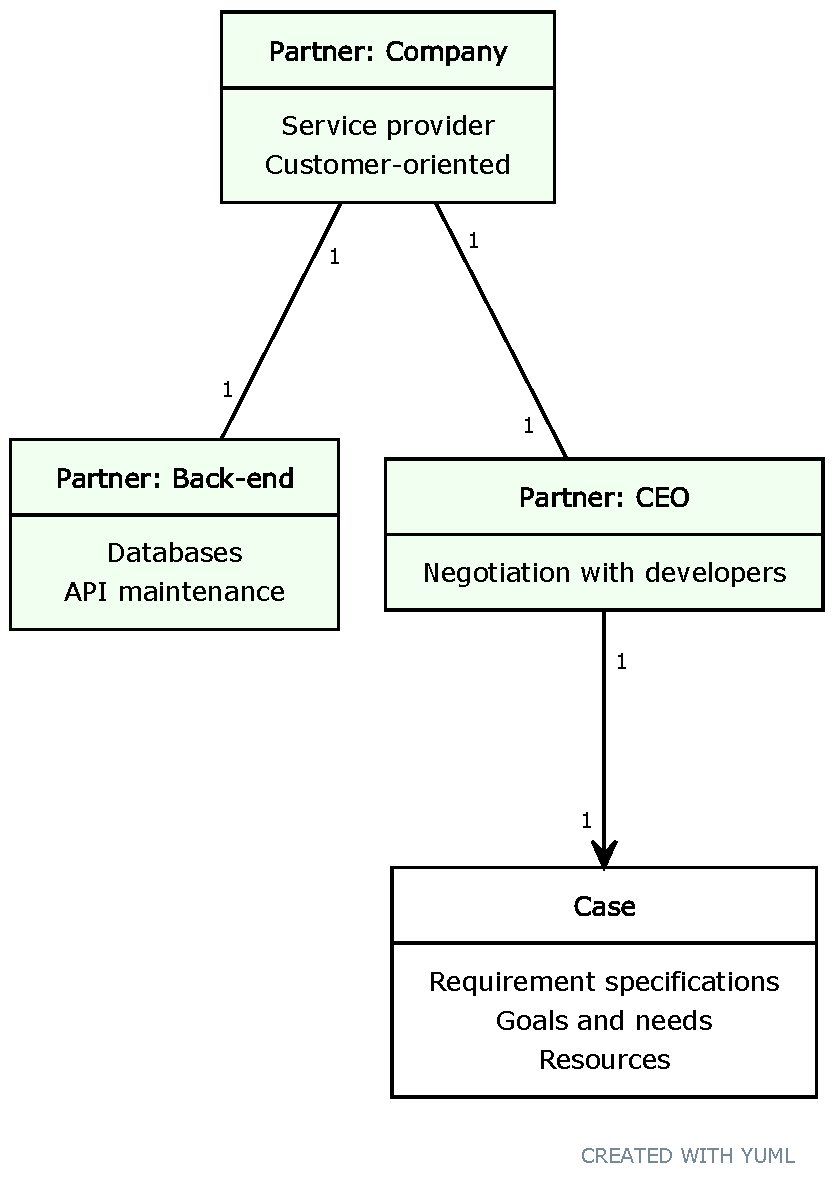
\includegraphics[width=0.8\linewidth]{figures/umlpartner.pdf}
\vspace{0.5cm} \\
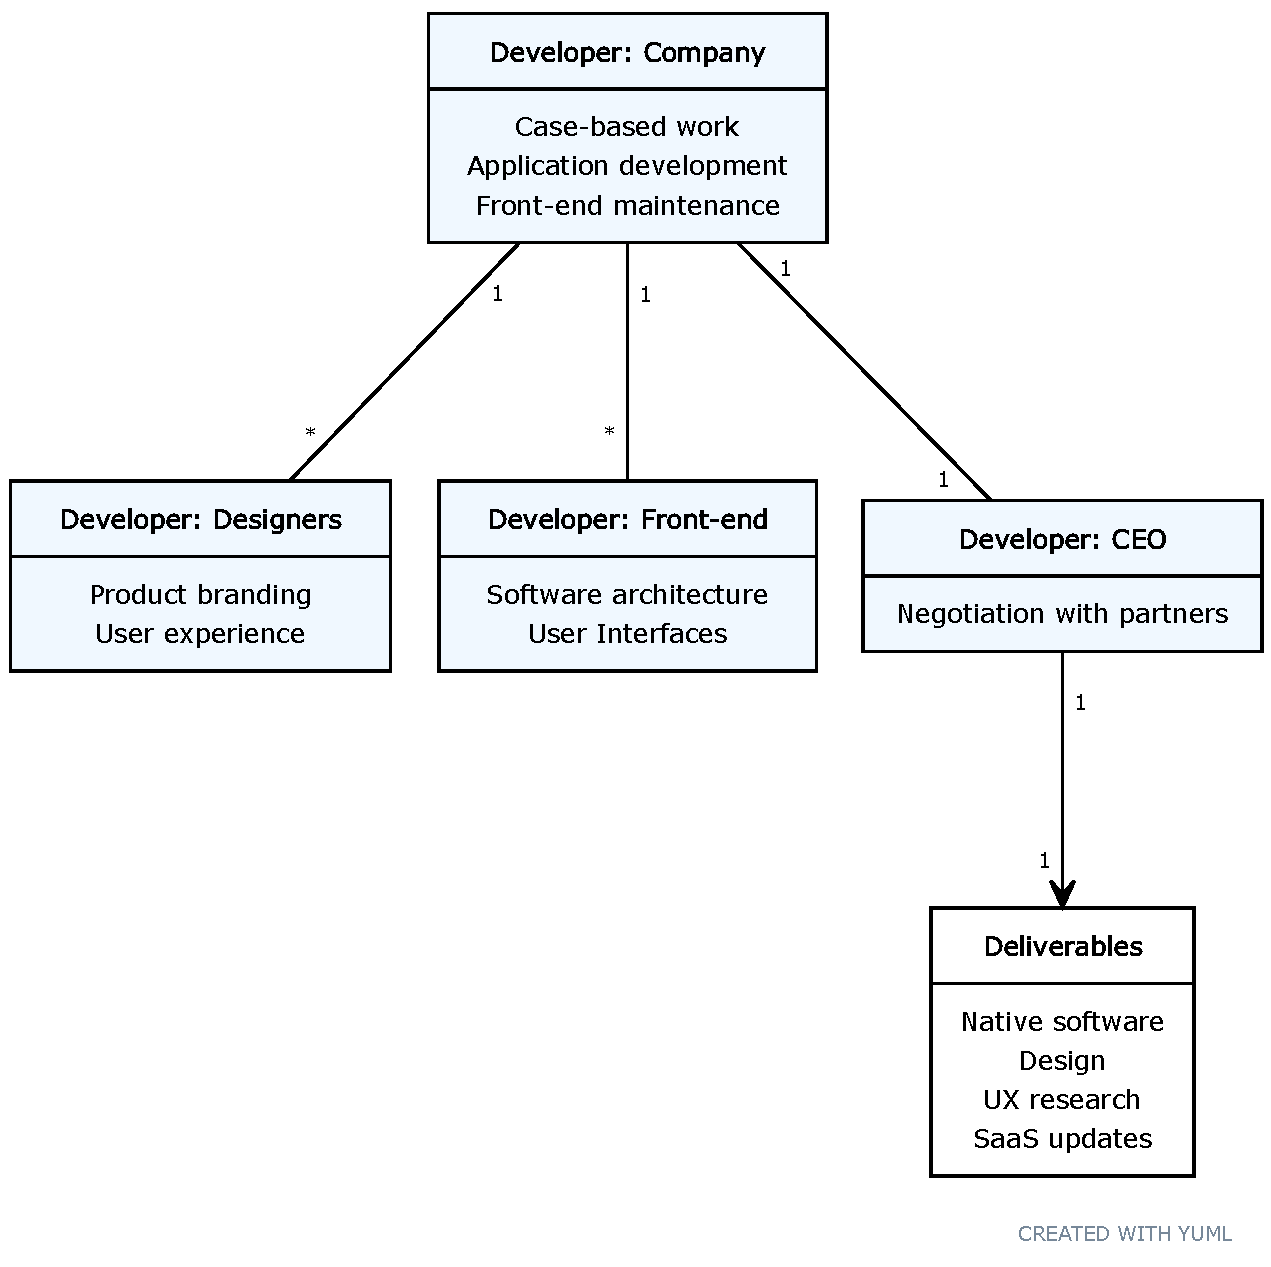
\includegraphics[width=0.8\linewidth]{figures/umldeveloper.pdf}
\caption{Hierarchical and structural relationship between development company and case partners.}
\label{fig:organisation}
\end{figure}

The structure of the partner company informs how they formulate the case offered to the developers. They are also responsible for maintenance of a back-end, delivering customer data to the client developed in the delivery.

The structure of the development company informs how they plan and execute on a case. They are not responsible for the back-end, and thus have to negotiate infrastructure plans and changes with their partners. This presents challenges to their autonomy, hierarchy and responsibilities.

\subsection{Perspectives on serialised data}

This section presents the personas derived from interviews with each development team at the company, for the purpose of taking value-oriented design decisions derived from their perspectives. As these employees are coworkers, their perspectives are grounded in shared experiences, yet their unique deviations highlight how serialised data has varying implications on work practices.

\begin{figure*}
\def\arraystretch{1.5}
\centering
\begin{tabular}{|p{0.3\linewidth}|p{0.5\linewidth}|}
\hline
Feature & Description \\
\hline
... & ... \\ 
... & ... \\ 
... & ... \\ 
\hline
\end{tabular}
\vspace{0.5cm} \\
\begin{tabular}{|p{0.3\linewidth}|p{0.5\linewidth}|}
\hline
Feature & Description \\
\hline
... & ... \\ 
... & ... \\ 
... & ... \\ 
\hline
\end{tabular}
\caption{Personas.}
\label{fig:personas}
\end{figure*}

\end{document}